\newgeometry{top=3cm, bottom=2cm}
\chapter{Results and discussion}
\label{chapter:results}

This chapter covers the results and analysis of the case study with discussion to related research.
First the results of interview for demographic purposes are
presented. Second, survey and interview results regarding JUnit compared to Spock and Spectrum are analyzed.  Third, the test
code analysis is presented and finally
with all the above mentioned results, Spock and Spectrum are compared against each other.

\section{First interview: demographics and projects}
\label{section:demographics}
    First interview was conducted to study about the demographics of participants and projects under research.
    The demographics of participants are displayed in table \ref{tab:demographics}. To summarize the
    participants, all can be categorized as senior software developers with many years of working with \textit{xUnit testing family} frameworks.
    Only participant C has a fair amount of prior experience working with BDD testing frameworks.
    \begin{table}[H]
        \resizebox{\textwidth}{!}{%
            \begin{tabular}{p{8.0cm}*{3}{p{3.5cm}}}
            \headcol & & &  \\
            \headcol {\large\textbf{Participant attribute}} & {\large\textbf{Participant A}} & {\large\textbf{Participant B}} & {\large\textbf{Participant C}} \\
            \hline
            \rowcol & & & \\
            \rowcol \textbf{Project} & Project A & Project A & Project B \\ \hline
            & & & \\
            \textbf{Software development experience} & 17 years & 15 years & 8 years \\ \hline
            \rowcol & & &  \\
            \rowcol \textbf{Java development experience} & 14 years & 1 year & 5-6 years  \\ \hline
            & & &  \\
            \textbf{Spring Framework experience} & 7 years & 1 year & 5-6 years \\ \hline
            \rowcol & & &  \\
            \rowcol \textbf{Automated unit testing experience} & 14 years; & 10 years; & 3-4 years; \\
            \rowcol \multicolumn{1}{r}{\textit{with frameworks}\textcolor{white}{-------------}} & \textit{JUnit} & \textit{CPPUnit, JUnit} & \textit{JUnit, TestNG} \\ \hline
            & & &  \\
            \textbf{Automated integration testing \newline experience} & 14 years; & Hardly at all; & 5-6 years; \\
            \multicolumn{1}{r}{\textit{with frameworks}\textcolor{white}{------------}} & \textit{JUnit, Some Robot Framework with Selenium} & \textit{JUnit} & \textit{JUnit, TestNG} \\ \hline
            \rowcol & & &  \\
            \rowcol \textbf{BDD testing framework experience} & \textless \textit{ } 1 year; & - & 2-3 years; \\
            \rowcol \multicolumn{1}{r}{\textit{with frameworks}\textcolor{white}{------------}} & \textit{Jasmine, Mocha} & & \textit{JBehave} \\
            \rowcol & & &  \\ \bottomlinec
            \end{tabular}}
            \caption {Participant demographics} \label{tab:demographics}
    \end{table}
\restoregeometry

The projects under study can both be categorized as web application projects with Java \textit{Spring Framework} backend technology.
They both have an agile development process. \textbf{Project A} is a customer project in public administration context.
\textbf{Project B} is an in-house project. They are both on the medium scale in code size, but financially project A can be
categorized as medium to large category.

Project A has two developers, \textbf{participants A} and \textbf{B}, working with Spring Framework backend,
where there is automated low-level testing in place with \textit{JUnit}.
Project B has only one backend developer, \textbf{participant C}, working with Spring Framework. As Project B
was developed in larger scale from 2012 to 2013 and published originally in 2013, it has some of the automated
low-level testing with JUnit done by others than participant C. Still most of this kind of test work is done by participant C.
Table \ref{tab:projects} displays the details of projects A and B.
    \begin{table}[H]
        \resizebox{\textwidth}{!}{%
            \begin{tabular}{p{7.5cm}*{2}{p{6cm}}}
            \headcol & & \\
            \headcol {\large\textbf{Project attribute}} & {\large\textbf{Project A}} & {\large\textbf{Project B}} \\ \hline
            \rowcol & &  \\
            \rowcol \textbf{Description} & Web application for area management, replacing existing system & Wep application for working hours tracking \& reporting \\ \hline
            & &   \\
            \textbf{Context} & Public administration, development for customer & In-house develoment \\ \hline
            \rowcol & & \\
            \rowcol \textbf{Development process} & Agile development with customized \textit{Scrum} & Agile with loosely defined process \\ \hline
            & &  \\
            \textbf{Size \& development team} & Medium - large project; \newline 3 developers for approximately 1,5 years & Small - medium project; \newline Published 2013, now 2 developers maintaining \& further development \\ \hline
            \rowcol & & \\
            \rowcol \textbf{Architecture} & Client rendered single-page \newline application & Server MVC with some client rendered views \\ \hline
            & & \\
            \textbf{Technologies} & \textit{Java Spring Boot \& Angular 2} & \textit{Java Spring Framework \& JSP, Backbone.js} \\ \hline
            \rowcol & & \\
            \rowcol \textbf{Quality assurance process} & Automated unit \& integration testing, code reviews, continuous integration, no dedicated tester & Automated unit, integration \& acceptance testing, code reviews, continuous integration, no dedicated tester \\ \hline
            & & \\
            \textbf{Used unit testing framework} & \textit{JUnit} & \textit{JUnit} \\ \hline
            \rowcol & &  \\
            \rowcol \textbf{Used integration testing framework} & \textit{JUnit} extended for \textit{Spring Framework} & \textit{JUnit} extended for \textit{Spring Framework} \\\hline
            \textbf{Chosen BDD testing framework} & \textit{Spectrum} & \textit{Spock} \\
            & &  \\ \bottomlinec
            \end{tabular}}
            \caption {Project details} \label{tab:projects}
    \end{table}

\section{Surveys and BDD framework feedback interview analyzed}
This section covers the results analyzed for both JUnit and BDD framework surveys together with participant BDD framework feedback interviews.
First the developer practices and their changes are answered with the data. Second, developer perception of low-level
testing and its changes are illustrated. Together these sections answer RQ1 \& and RQ2.

The baseline for answers was conducted with the survey described in detail in Appendix \ref{chapter:surveys} section \ref{section:junit-survey}.
These questions related to JUnit low-level testing are displayed with \textbf{Q1, Q2, Q3} and so on. Their counterparts, questions aimed to study the changes
in low-level testing with new BDD implementation level testing framework are marked as \textbf{Q1', Q2', Q3'} and so on. Details
of BDD surveys can be found in Appendix \ref{chapter:surveys} section \ref{section:bdd-survey}. Participants whom answered
the surveys were {\colorbox{lightgray}A}, {\colorbox{lime}B} and {\colorbox{orange}C}. The color coding of participants is
visible throughout the result tables for easier highlighting of answers.

\subsection{Automated low-level testing developer practices}
This section answer the
\textbf{RQ1: }\textit{How does behavior-driven testing frameworks change developer practices working with automated
low-level testing compared to JUnit framework?} This is studied through multiple aspects, which all display results and analysis
individually. First, the developer software development \& testing time and effort usage is analyzed. Second, low-level
test optimizing targets are inspected. Third, test understandability and informativiness is under study. After that, test
refactoring techniques and commenting practices are analyzed. Finally, unit testing practices are studied in more detail
before summarizing the answers to RQ1 and the changes in low-level testing developer practices.

\subsubsection{Software development \& testing time and effort usage}
    \begin{figure}[ht]%
        \centering
        \subfloat[Results in original study~\cite{daka2014survey} ]{{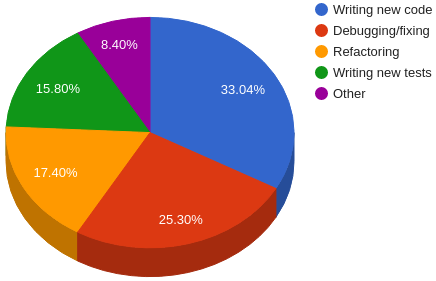
\includegraphics[width=6.75cm]{images/org-time.png} }}%
        \qquad
        \subfloat[Results in this study]{{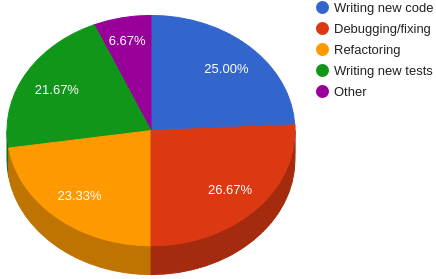
\includegraphics[width=6.75cm]{images/new-time.png} }}%
        \caption{Developer software development time usage}%
        \label{fig:time-usage}%
    \end{figure}
First studied aspect of developer practices was \textbf{time usage}. Figure \ref{fig:time-usage} displays the developer software development time usage
in original study~\cite{daka2014survey} and in this thesis. Table \ref{tab:changes-pt1a} display the participant values
also individually and the changes in time usage after the introduction of a new BDD framework. In the original study, writing
new code is the dominating activity in time usage with 33.04\% share. At the beginning of this study when studying JUnit practices,
participants used most of their software development
time in \textit{debugging or fixing} activities with 26.67\% time usage share. \textit{Writing new code} (25.00\%) and \textit{refactoring} (23.33\%) were close
by in time usage. The participants in this study had quite much variance in their answers for time usage, but \textit{writing
new tests} was uniformly higher in time usage than in the original study results. Participants A and C
were closely together in their answers for time usage, whereas participant B had more emphasis on initial \textit{writing of new code} and
less time spent on \textit{refactoring}.

    \begin{table}[H]
        \resizebox{\textwidth}{!}{%
            \begin{tttabular}{p{8.0cm}*{7}{p{1.7cm}}}
            \topline
            \textbf{Question} & \textbf{Answer options} &  &  &  &   &  & \\ \hline
            \textbf{Q1: How do you spend your software development time (in percentages)} & Participant {\colorbox{lightgray}A} & Participant {\colorbox{lime}B} & Participant {\colorbox{orange}C} & Average & & \\
            & & & & & & & \\
            1. Writing new code & 20\% & 40\% & 15\% & 25\%  \\
            2. Writing new tests & 20\% & 25\% & 20\% & 21.67\% \\
            3. Debugging/fixing & 30\% & 25\% & 25\% & 26.67\% \\
            4. Refactoring & 20\%  & 10\% & 30\% & 23.33\% \\
            5. Other & 10\% & 0\% & 10\% & 6.67\% \\
            & \\ \hline
            \textbf{Q1': Compared to JUnit, How do you spend your software development time?} & A lot less time & Less time & Slightly less time & The Same amount of time & Slightly more time & More time & A lot more time \\
            & \\
            1. Writing new code & & & & {\colorbox{lightgray}A}{\colorbox{lime}B}{\colorbox{orange}C} & & & \\
            2. Writing new tests & & {\colorbox{orange}C} & & {\colorbox{lightgray}A} & {\colorbox{lime}B} & & \\
            3. Debugging/fixing & & & & {\colorbox{lightgray}A}{\colorbox{lime}B}{\colorbox{orange}C} & & & \\
            4. Refactoring & & & {\colorbox{orange}C} & {\colorbox{lightgray}A}{\colorbox{lime}B} & & & \\
            5. Other & & & & {\colorbox{lightgray}A}{\colorbox{lime}B}{\colorbox{orange}C} & & & \\
            & \\ \topline


            \end{tttabular}}
            \caption {Development time usage and changes in it} \label{tab:changes-pt1a}
    \end{table}

Changes in software development time were studied with the \textbf{Q1':} \textit{Compared to JUnit, How do you spend your
software development time?} Results are displayed in table \ref{tab:changes-pt1a}. Participant A
didn't see any changes in the overall software development time usages after introduction of \textbf{\textit{Spectrum}}. This has to be taken
with a grain of salt, as the  next questions shows increase in testing efforts when comparing JUnit and Spectrum.
Participant B noticed a slight increase in time used to write new tests with Spectrum, whereas other time usages remained
the same. On the other hand, participant C said to use less time writing new tests and slightly less time refactoring the code with Spock.
These testing time usages are analyzed in detail with Q2'.

Questions \textbf{Q2} and \textbf{Q2'} further analyze the time usage, now focusing in automated testing. Their results are
shown in table \ref{tab:changes-pt1b}. All participants answered to use approximately 30 minutes of time in single test case. The
averages show that about one third (28.33\%) of initial effort goes to \textit{thinking} about the test case without actual implementation.
About two thirds (71.67\%) of initial effort goes to \textit{implementation} of the test case. \textit{Refactoring} takes about one third (28.33\%)
of the overall testing effort.

Participants had highly varying answers in initial \textit{thinking} and \textit{implementation} effort and also
in overall testing \textit{refactoring} effort. Participants B and C had same kind of profile
in initial efforts, where about one fifth of it goes to initial \textit{thinking} of test case and four fifths to \textit{implementation}.
Participant A had the initial effort going in half between the two aspects. In overall effort,
\textit{refactoring} of test code took 50\% of effort for participant A. Participant B
hardly at all \textit{refactored} test code (5\%) and participant C used around one third of overall testing effort
to \textit{refactoring} (30\%).


    \begin{table}[H]
        \resizebox{\textwidth}{!}{%
            \begin{tttabular}{p{8.0cm}*{7}{p{1.7cm}}}
            \topline
            \textbf{Question} & \textbf{Answer options} &  &  &  &   &  & \\ \hline
            \textbf{Q2: How do you spend your low-level automated testing time} & Participant {\colorbox{lightgray}A} & Participant {\colorbox{lime}B} & Participant {\colorbox{orange}C} & Average & & \
            & & & & & & & \\
            1. How much approximately you use time per test case (minutes)? & 30 min & 30 min & 30 min & 30 min \\
            2. How much of your initial effort goes to thinking about test case content without implementation? & 50\% & 20\% & 15\% & 28.33\% \\
            3. How much of your initial effort goes to initial test case structuring and implementation? & 50\% & 80\% & 85\% & 71.67\% \\
            4. How much of your overall testing effort goes to refactoring test code (percentage)? & 50\% & 5\% & 30\% & 28.33\% \\
            & \\ \hline
            \textbf{Q2': Compared to JUnit, How do you spend your low-level automated testing time?} & A lot less & Less & Slightly less & The Same amount & Slightly more & More & A lot more \\
            & \\
            1. Do you use more or less time per test case? & & {\colorbox{orange}C} & & {\colorbox{lightgray}A} & {\colorbox{lime}B} & & \\
            2. Do you use more or less of initial effort thinking about test case content? & & & & {\colorbox{orange}C} & {\colorbox{lightgray}A}{\colorbox{lime}B} & & \\
            3. Do you use more or less of initial effort to test case structuring and implementation? & & & & {\colorbox{orange}C} & {\colorbox{lime}B} & {\colorbox{lightgray}A} & \\
            4. Do you use more or less of overall testing effort to refactoring test code? & & & {\colorbox{orange}C} & {\colorbox{lightgray}A} & {\colorbox{lime}B} & & \\
            & \\ \topline

            \end{tttabular}}
            \caption {Development \& testing time and effort usage and changes in them} \label{tab:changes-pt1b}
    \end{table}

Changes in automated testing time and effort were studied with \textbf{Q2':} \textit{Compared to JUnit, How do you spend your low-level automated testing time?}
Participant A answered
to use around the same time per test case with Spectrum, but also answered to use slightly more effort in initial \textit{thinking} of test
case and more effort in test case \textit{implementation}. The overall test \textit{refactoring} effort was the same amount. All effort changes combined, it might
be feasible to think that the time per test case might have increased. In the feedback interview of \textbf{\textit{Spectrum}} with participant
A, he said that the implementation and how to effectively structure the usage of Java 8 lambdas and Spectrum variables
in them took extra time compared to JUnit. Participant B asnwered to use slightly more time with Spectrum on all aspects of low-level testing.
In the followed interview, this was found out to be caused by in general the new testing framework and especially the lambda structure
of tests with it. Participant C answered to use less time per test case with slightly less effort on test refactoring. In the
following interview, participant C answered that it was quick to feel effective with Spock and especially its DDT allowed to
easily test out different situations.

In conclusion, Spectrum seems to have a longer learning curve than Spock. Participants A and B both said in interview that it still
feels like there is learning to do to be effective with Spectrum. Participant C had previously used JBehave which also
uses the same \textit{Gherkin}-structure as Spock, therefore it might have eased the introduction of Spock for him. Survey
results also support this. After two months, testing with Spectrum seems to take more effort and time than with JUnit.

\subsubsection{Test optimizing targets}

    \begin{figure}[H]
      \begin{center}
        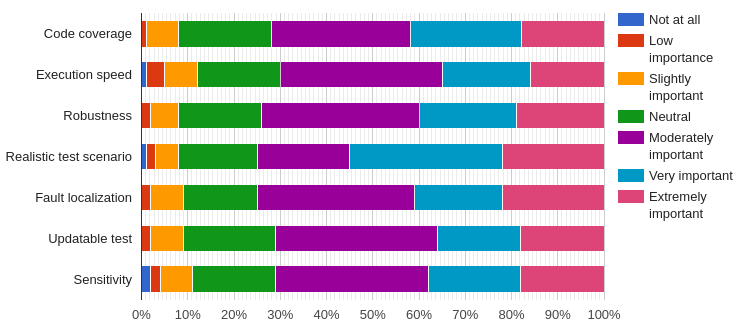
\includegraphics[width=14.7cm]{images/optimize-org.png}
        \caption{Original study~\cite{daka2014survey} unit test optimizing target percentages amongst developers}
        \label{fig:org-optimize}
      \end{center}
    \end{figure}
Original study by Daka and Fraser~\cite{daka2014survey} studied unit testing \textbf{optimizing targets} for tests. Figure \ref{fig:org-optimize}
displays the results from original study. All the studied aspects had at least over 60\% of developers finding them ranging
from moderately important to extremely important. \textit{Realistic test scenario} was the most important optimizing target
amongst original study survey participants.


Regarding JUnit low-level testing, participants in this study had varying importance in studied aspects. Full answers are
displayed in table \ref{tab:changes-pt2} with \textbf{Q3:} \textit{How important are the following aspects for you when you write new low-level tests?}
Participants A and B answered
the most alike, whereas participant C had slightly different optimizing profile. \textit{Code coverage}
was a neutral optimizing target for all participants. Additional question original to this study was the \textit{capturing of behavior}
as optimizing target. Participants A and B found it neutral and slightly important,
but participant C had it as a very important optimizing target. Another interesting target was \textit{execution speed},
where participants A and B had it at least moderately important, but participant C
answered it as low importance optimizing target. \textit{How realistic the test scenario is} was very important to optimize for
participant C. This was also the most important target amonst original study survey participants.
For participants A and B, \textit{realistic test scenario} was only slightly important.
These kind of variations in optimizing targets are quite natural when studying this low participant count. The original study
figure \ref{fig:org-optimize} displays how all the targets are quite close to each other with larger sampling.

    \begin{table}[H]
        \resizebox{\textwidth}{!}{%
            \begin{tttabular}{p{8.0cm}*{7}{p{1.7cm}}}
            \topline
            \textbf{Question} & \textbf{Answer options} &  &  &  &   &  & \\ \hline
            \textbf{Q3: How important are the following aspects for you when you write new low-level tests?} & Not at all & Low \newline importance & Slightly important & Neutral & Moderately important & Very \newline important & Extremely important \\
            & \\
            1. Code coverage & & & & {\colorbox{lightgray}A}{\colorbox{lime}B}{\colorbox{orange}C} & & & \\
            2. Capturing all behavior of unit/feature with tests or assertions & & & {\colorbox{lime}B} & {\colorbox{lightgray}A} & & {\colorbox{orange}C} & \\
            3. Execution speed & & {\colorbox{orange}C} & & & {\colorbox{lime}B} & {\colorbox{lightgray}A} & \\
            4. Robustness against code changes (i.e., test does not break easily) & & & & & {\colorbox{lightgray}A}{\colorbox{lime}B}{\colorbox{orange}C} & & \\
            5. How realistic the test scenario is & & & {\colorbox{lightgray}A}{\colorbox{lime}B} & & & {\colorbox{orange}C} & \\
            6. How easily faults can be localised/debugged if the test fails & & & {\colorbox{lime}B} & & {\colorbox{lightgray}A}{\colorbox{orange}C} & & \\
            7. How easily the test can be updated when the underlying code changes & & {\colorbox{orange}C} & {\colorbox{lightgray}A} & & {\colorbox{lime}B} & & \\
            8. Sensitivity against code changes (i.e., test should detect even small code changes) & & {\colorbox{lightgray}A}{\colorbox{lime}B} & & {\colorbox{orange}C} & & & \\
            & \\ \hline
            \textbf{Q3': Compared to JUnit, How important are the following aspects for you when you write new low-level tests?} & A lot less important & Less important & Slightly less important & As important as before & Slightly more important & More important & A lot more important \\
            & \\
            1. Code coverage & & & & {\colorbox{lightgray}A}{\colorbox{lime}B}{\colorbox{orange}C} & & & \\
            2. Capturing all behavior of unit/feature with tests or assertions & & & & {\colorbox{lime}B}{\colorbox{orange}C} & {\colorbox{lightgray}A} & & \\
            3. Execution speed & & & & {\colorbox{lightgray}A}{\colorbox{lime}B}{\colorbox{orange}C} & & & \\
            4. Robustness against code changes (i.e., test does not break easily) & & & & {\colorbox{lightgray}A}{\colorbox{lime}B}{\colorbox{orange}C} & & & \\
            5. How realistic the test scenario is	& & & & {\colorbox{lightgray}A}{\colorbox{lime}B} & & {\colorbox{orange}C} & \\
            6. How easily faults can be localised/debugged if the test fails & & & & {\colorbox{lime}B} & {\colorbox{lightgray}A}{\colorbox{orange}C} & & \\
            7. How easily the test can be updated when the underlying code changes & & & & {\colorbox{lightgray}A}{\colorbox{lime}B}{\colorbox{orange}C} & & & \\
            8. Sensitivity against code changes (i.e., test should detect even small code changes) & & & & {\colorbox{lightgray}A}{\colorbox{lime}B}{\colorbox{orange}C} & & & \\
            & \\ \topline

            \end{tttabular}}
            \caption {Optimizing targets in low-level tests and changes in them} \label{tab:changes-pt2}
    \end{table}

The changes in low-level testing optimizing targets were studied with \textbf{Q3':}
\textit{Compared to JUnit, how important are the following aspects for you when you write new low-level tests?}
Participant A compared the changes from JUnit to \textbf{\textit{Spectrum}} and find most of the targets as important as before.
\textit{Capturing behavior} of tested subject in tests was slightly more important than before. Also \textit{fault localization} was
slightly more important target than before. These two targets and their higher importance seem natural for a \textbf{xSpec family}
testing framework, as it aims to promote more granular and more natural language description information holding test cases than JUnit.
Participant B didn't feel there to be any optimizing target changes. In the interview he stated that none of the targets
really changed one way or another for him when using Spectrum instead of JUnit.

Participant C found \textit{realistic test
scenario} to be more important with Spock than it was with JUnit. Realistic test scenario was already very important for him
with JUnit and with Spock, it is even more important. He also answered \textit{easy fault localization} to be slightly
more important than before. In the interview it was found out that these aspects had more importance because of the BDD-style of writing
the tests with Spock. For participant C, \textit{capturing behavior} with tests was already very important with JUnit and it was
interesting that Spock didn't change this. The \textit{COTM}-metric with JUnit in test code analysis section shows support
for already granular unit test cases in project B and this might act as an indicator of already behaviorally described test methods.

To conclude, its hard to see any pattern in test optimizing target changes. Altogether, the changes were quite mild.
Easier fault localization was the only common nominator that was found slightly more important with two out of three
participants. Therefore it might be feasible to say, that test optimizing targets aren't too tied to the testing framework in this study context.
This might show different results with larger sampling repeating the same kind of study. The results might be different especially when using these
implementation level BDD-testing frameworks for actual practicing of BDD. Then the optimizing targets might be much different
than with \textbf{xUnit family} testing.

\subsubsection{Test understandability and informativeness }

    \begin{figure}[H]
      \begin{center}
        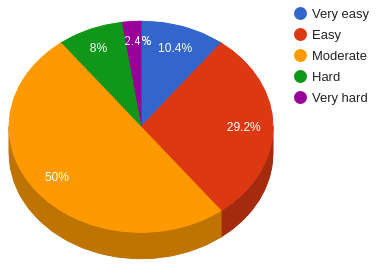
\includegraphics[width=7.7cm]{images/org-understandability.png}
        \caption{Original study~\cite{li2016automatically} unit test understandability}
        \label{fig:org-understandability}
      \end{center}
    \end{figure}

The difficulty of developers \textbf{understanding} unit tests was studied by Li et al.~\cite{li2016automatically}. Over 60\% of survey
participants found it at least moderately difficulty. Figure \ref{fig:org-understandability} illustrates the total survey
answer regarding unit test understandability. This question was chosen to be replicated in this study to see, if the research
hypothesis of developers finding it easier to understand test cases with BDD testing frameworks will hold true.

Table \ref{tab:changes-pt3} summarizes this study participant answers. First \textbf{Q4} studied how difficult understanding
of low-level tests with JUnit was. The results mirrored quite well the original study findings, as participants B and C
find the understandability to be moderately difficult and participant A found it hard to understand a low-level test.


    \begin{table}[H]
        \resizebox{\textwidth}{!}{%
            \begin{tttabular}{p{8.0cm}*{7}{p{1.7cm}}}
            \topline
            \textbf{Question} & \textbf{Answer options} &  &  &  &   &  & \\ \hline
            & Very easy & Easy & Moderate & Hard & Very hard & & \\
            & \\
            \textbf{Q4: How difficult is it for you to understand a low-level test?} & & & {\colorbox{lime}B}{\colorbox{orange}C} & {\colorbox{lightgray}A} & \\
            & \\ \hline
            & A lot less difficult & Less difficult & Slightly less difficult & As difficult as before & Slightly more difficult & More difficult & A lot more difficult \\
            & \\
            \textbf{Q4': Compared to JUnit, how difficult is it for you to understand a low-level test?} & {\colorbox{orange}C} & {\colorbox{lightgray}A} & & & {\colorbox{lime}B} & & \\
            & \\ \topline
            \end{tttabular}}
            \caption {Understandability of low-level tests and changes in it} \label{tab:changes-pt3}
    \end{table}

The changes in low-level test understandability were studied with \textbf{Q4':} \textit{Compared to JUnit, how difficult is it
for you to understand a low-level test?} Participant A found it less difficult to understand a low-level
test after the introduction of \textbf{\textit{Spectrum}}. Participant B find it slightly more difficult to understand
a low-level test. This was further analyzed with interview, where he says that the divided nested structure of Spectrum
files make it slightly harder to understand individual tests as whole. Compared to JUnit, Participant C found it a lot less difficult to
understand Spock tests. In the interview this was further inspected and he states that its much more easier to write
information to Spock feature methods compared to JUnit test methods.

Summing up, participant surveys and interviews seem to support partially the \textbf{H2:} \textit{"Developers will find it easier to understand test cases"}.
Although, participant B find it slightly harder to understand low-level tests at times, there is still more evidence for
easier undestanding. H2 is further studied with following questions in this section.

Table \ref{tab:changes-pt4} displays questions \textbf{Q5 \& Q5'} and their results. Q5 was chosen to see
how easily the JUnit test methods can be \textbf{structured} and \textbf{understood} to hold different parts of the test. JUnit testing literature states that
the structure should be done with \textit{Arrange-Act-Assert}~\cite{langr2015pragmatic}, but it is not enforced and thus can lead to poorly structured
tests which are hard to understand~\cite{kapelonis2016java}. Q5 studies if this does hold true.

All the participants had different parts of test
structure with ranging difficulties in structuring and understanding. Participant A could be categorized to hold almost all
parts of structuring the test somewhat difficult, with the exception of finding it easy to structure information to context of tests.
Reading tests and understanding their structure was found at least from slightly hard to hard.
Participant B find writing information to assertions of test easy, but otherwise structuring the test
was found from moderately difficult to slightly hard. Reading the test structure parts for information was equivalent
to writing and structuring of tests. Participant C found it somewhat difficult to produce information
to tests, but reading the test structure was found to be slightly easy. These ranging results are not too surprising,
as JUnit does not promote a certain structure for tests. It seems to result in hard to produce stucture that is not
too easy to understand.

    \begin{table}[H]
        \resizebox{\textwidth}{!}{%
            \begin{tttabular}{p{8.0cm}*{7}{p{1.7cm}}}
            \topline
            \textbf{Question} & \textbf{Answer options} &  &  &  &   &  & \\ \hline
            \textbf{Q5: In low-level testing, how difficult is it for you to} & Very easy & Easy & Slightly easy & Moderate & Slightly hard & Hard & Very hard \\
            & & & & & & \\
            1. Structure and write information to context of test? & & {\colorbox{lightgray}A} & & & {\colorbox{lime}B}{\colorbox{orange}C} & & \\
            2. Structure and write information to stimulus of test? & & & & {\colorbox{lightgray}A}{\colorbox{lime}B}{\colorbox{orange}C} & & & \\
            3. Structure and write information to assertions of test? & & {\colorbox{lime}B} & {\colorbox{orange}C} & & {\colorbox{lightgray}A} & & \\
            4. Read test case structure for information about context of test? & & & {\colorbox{orange}C} & & {\colorbox{lime}B} & {\colorbox{lightgray}A} & \\
            5. Read test case structure for information about stimulus of test? & & & {\colorbox{orange}C} & {\colorbox{lime}B} & {\colorbox{lightgray}A} & & \\
            6. Read test case structure for information about assertions of test? & & {\colorbox{lime}B} & {\colorbox{orange}C} & & & {\colorbox{lightgray}A} & \\
            & \\ \hline
            \textbf{Q5': Compared to JUnit in low-level testing, how difficult is it for you to} & A lot less difficult & Less difficult & Slightly less difficult & As difficult as before & Slightly more difficult & More difficult & A lot more difficult \\
            & & & & & & \\
            1. Structure and write information to context of test? & {\colorbox{lightgray}A}{\colorbox{orange}C} & & {\colorbox{lime}B} & & & & \\
            2. Structure and write information to stimulus of test? & & {\colorbox{lightgray}A}{\colorbox{orange}C} & & & {\colorbox{lime}B} & & \\
            3. Structure and write information to assertions of test? & & {\colorbox{orange}C} & {\colorbox{lightgray}A} & {\colorbox{lime}B} & & & \\
            4. Read test case structure for information about context of test? & {\colorbox{orange}C} & & {\colorbox{lightgray}A}{\colorbox{lime}B} & & & & \\
            5. Read test case structure for information about stimulus of test? & & {\colorbox{lightgray}A}{\colorbox{orange}C} & & {\colorbox{lime}B} & & & \\
            6. Read test case structure for information about assertions of test? & & {\colorbox{orange}C} & {\colorbox{lightgray}A}{\colorbox{lime}B} & & & & \\
            & \\ \topline
            \end{tttabular}}
            \caption {Low-level test structure informativiness and changes in it} \label{tab:changes-pt4}
    \end{table}

Q5' displays the changes in structuring and reading of tests for information. Participant A found \textbf{\textit{Spectrum}}
on all occasions easier to structure information to tests and also to read it from tests. Structuring information to
tests could be categorized as quite much easier. Reading the tests for information was found somewhat easier than with JUnit.
Participant B found the changes in structuring of tests with Spectrum to range from slightly less difficult to slightly
more difficult, but the reading of test case structure could be summed up to be somewhat more easier than with JUnit.
In the interview he said that the main benefits of Spectrum was the easier spotting of different parts of test. Participant
C found it ranging from less to a lot less difficult structuring and reading the tests.

In conclusion, the results show that \textit{structuring} and \textit{reading} of the different parts of tests was found almost unanimously \textbf{more easier}
with BDD-testing frameworks than with JUnit. This finding supports the \textbf{H2}, but for more evidence, the next
questions Q6 and Q6' need to be analyzed.

Table \ref{tab:changes-pt5} displays questions \textbf{Q6 \& Q6'} with results. First Q6 studies how \textbf{informative} participants
found JUnit test output. Participant A find the output hardly informative, whereas participants B
and C found the output ranging from somewhat informative to moderately informative. These results are
not too suprising, as normal JUnit test method naming do not tend hold that much words. Section \ref{subsub:low-level-metrics} displays
that the average word count in test methods in projects were ranging from approximately 5 to 6. This amount of words can't
hold naturally too much information in total.

    \begin{table}[H]
        \resizebox{\textwidth}{!}{%
            \begin{tttabular}{p{8.0cm}*{7}{p{1.7cm}}}
            \topline
            \textbf{Question} & \textbf{Answer options} &  &  &  &   &  & \\ \hline
            & Not at all & Hardly informative & Slightly informative & Somewhat informative & Moderately informative & Very informative & Extremely informative \\
            & \\
            \textbf{Q6: How informative you usually find the test output?} & & {\colorbox{lightgray}A} & & {\colorbox{orange}C} & {\colorbox{lime}B} & & \\
            & \\ \hline
            & A lot less informative & Less informative & Slightly less informative & As informative as before & Slightly more informative & More informative & A lot more informative \\
            & \\
            \textbf{Q6': Compared to JUnit, how informative you usually find the test output?} & & & & {\colorbox{lime}B} & {\colorbox{lightgray}A} & {\colorbox{orange}C} & \\
            & \\ \topline

            \end{tttabular}}
            \caption {Low-level test output informativeness and changes in it} \label{tab:changes-pt5}
    \end{table}

Q6' studies the change of test output informativeness after the introduction of new BDD testing framework. Participant A
found a slight increase in informativeness of output. Participant B found the output as informative as before, whereas participant
C found it more informative. As the \textbf{xSpec family} testing frameworks allow free text description to their
code example groups and code examples, the answer of participant B was further studied in interview. He stated that
he usually only checks from the output whether test passes or fails and as such doesn't see\newgeometry{bottom=1cm}\noindent any improvement when
comparing Spectrum and JUnit.

On the whole, it seems that \textbf{H2:} \textit{"Developers will find it easier to understand test cases"} has strong
evidence to support it. However, the results of questions Q4'-Q6' are not clear-cut unanimous and especially the nested structure of \textbf{xSpec family}
code example groups might not be so clear at the beginning. In any case, it can be concluded that BDD testing
frameworks allow to structure the tests for separate parts, which helps in identifying \textit{context, action}
and \textit{assertions} more explicitly from tests.

\subsubsection{Test code repetition reducing techniques}

Table \ref{tab:changes-pt6} displays the usage of different \textbf{repetition reducing} techniques. First \textbf{Q7:}
\textit{How much are the following repetition reducing techniques used in your low-level testing?} studies how much a
set of common refactoring techniques stated in unit testing literature ~\cite{artofunit2013} are used in projects.

Most common used refactoring techniques amongst survey participants were \textit{extract method} and lifecycle hook \textit{before -each}.
These two techniques were in use frequently or very frequently within participant testing. Lifecycle hook \textit{before -class} was also
in use at least occasionally. Automatic test generation through DDT was found very rarely or rarely used with participants A
and B. Section \ref{subsub:low-level-metrics} shows that in project A it was not used at all, where data-driven test method ratio to standard
low level test methods was 0. Participant C answered to use occasionally DDT and the test code analysis
data in section \ref{subsub:low-level-metrics} supported this. Common test initializer class inheritance was a practice
very rarely or rarely used amongst all participants. During interview, participant A even stated test class inheritance
to be \textit{"a practice to avoid, it's devil's work"}.

    \begin{table}[H]
        \resizebox{\textwidth}{!}{%
            \begin{tttabular}{p{8.0cm}*{7}{p{1.7cm}}}
            \topline
            \textbf{Question} & \textbf{Answer options} &  &  &  &   &  & \\ \hline
            \textbf{Q7: How much are the following repetition reducing techniques used in your low-level testing?} & Never & Very rarely & Rarely & Occasionally & Frequently & Very \newline frequently & Always \\
            & & & & & & \\
            1. Extract method (custom helper methods) & & & & & {\colorbox{lightgray}A}{\colorbox{lime}B} & {\colorbox{orange}C} & \\
            2. Lifecycle hooks Before/After (class) & & & & {\colorbox{orange}C} & {\colorbox{lightgray}A}{\colorbox{lime}B} & & \\
            3. Lifecycle hooks Before/After (each) & & & & & {\colorbox{lightgray}A}{\colorbox{lime}B} & {\colorbox{orange}C} & \\
            4. Automatic test generation via test method parametrization & & {\colorbox{lightgray}A} & {\colorbox{lime}B} & {\colorbox{orange}C} & & & \\
            5. Common test initializer class inheritance & & {\colorbox{lightgray}A}{\colorbox{orange}C} & {\colorbox{lime}B} & & & & \\
            & \\ \hline

            \textbf{Q7': Compared to JUnit, how much are the following repetition reducing techniques used in your low-level testing?} & A lot less & Less & Slightly less & The same amount & Slightly more & More & A lot more \\
            & & & & & & \\
            1. Extract method (custom helper methods) & & & {\colorbox{lime}B} & {\colorbox{lightgray}A}{\colorbox{orange}C} & & & \\
            2. Lifecycle hooks Before/After (class/all) & & & & {\colorbox{lightgray}A}{\colorbox{lime}B}{\colorbox{orange}C} & & & \\
            3. Lifecycle hooks Before/After (each) & & & & {\colorbox{lime}B}{\colorbox{orange}C} & & {\colorbox{lightgray}A} & \\
            4. Automatic test generation via test method parametrization & & & & {\colorbox{lightgray}A}{\colorbox{lime}B} & & & {\colorbox{orange}C} \\
            5. Common test initializer class inheritance & & & & {\colorbox{lightgray}A}{\colorbox{lime}B}{\colorbox{orange}C} & & & \\
            & \\ \topline

            \end{tttabular}}
            \caption {Used repetition reducing techniques for low-level testing and changes in their use} \label{tab:changes-pt6}
    \end{table}
\restoregeometry

\textbf{Q7':} \textit{Compared to JUnit, how much are the following repetition reducing techniques used in your low-level testing?}
studies how techniques are used differently with the new BDD testing framework to reduce repetition. Participant A
said to use techniques the same amount as before, with the exception of lifecycle hook \textit{before -each} being used more.
In the feedback interview, participant A stated that there was some confusion when to use \textit{before -all}
lifecycle hook and therefore hook \textit{before -each} was mainly used. The increased use of \textit{before -each} is
explained by the nested code example groups, which each support their own separate lifecycle hooks. Participant B used
the repetition reducing techniques the same amount, except for slightly less used \textit{extract method}. Participant
C answered to use \textit{automatic test generation via test method parametrization} (DDT) a lot more than before. Test
code analysis in section \ref{subsub:low-level-metrics} supports this claim.

In conclusion, both BDD testing frameworks allow new ways to reduce repetition in test code. How much they are used
seems to be independent on the developer. Later is studied how much more maintainable these techniques
make the test code in eyes of the participants.

\subsubsection{Test commenting practices}
    \begin{figure}[ht]%
        \centering
        \subfloat[Comment adding ]{{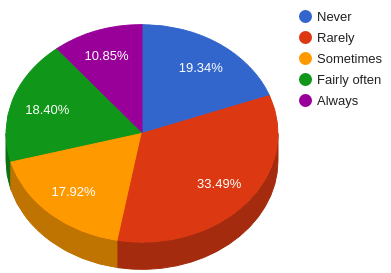
\includegraphics[width=6.75cm]{images/org-add-document.png} }}%
        \qquad
        \subfloat[Comment updating]{{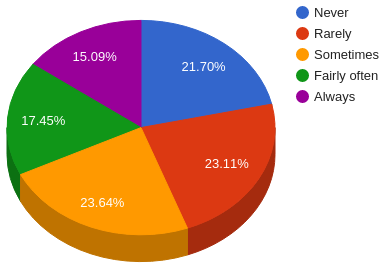
\includegraphics[width=6.75cm]{images/org-update-document.png} }}%
        \caption{Original study~\cite{li2016automatically} unit testing commenting practices}%
        \label{fig:org-commenting}%
    \end{figure}

Test commenting and comment updating was found to be a practice rarely done by most of the developers~\cite{li2016automatically}.
Figure \ref{fig:org-commenting} shows the original study results regarding test commenting practices. Participants in this
study seem to divide with commenting practices. Table \ref{tab:changes-pt7} displays the participant JUnit commenting practice results with
\textbf{Q8} and \textbf{Q9}. Project A and its participants A and B
answer fairly often to add and update comments in low-level test cases. Participant C rarely practices
test commenting or updating. Test data analysis in \ref{subsub:low-level-metrics} correlates with participant answers, as
project A had quite much commenting in test methods and project B very little.

    \begin{table}[H]
        \resizebox{\textwidth}{!}{%
            \begin{tttabular}{p{8.0cm}*{7}{p{1.7cm}}}
            \topline
            \textbf{Question} & \textbf{Answer options} &  &  &  &   &  & \\ \hline
            & Never & Rarely & Sometimes & Fairly often & Always & & \\
            & \\
            \textbf{Q8: How often do you add/write documentation comments to low-level test cases?} & & {\colorbox{orange}C} & & {\colorbox{lightgray}A}{\colorbox{lime}B} & \\
            & \\ \hline
            & A lot less & Less & Slightly less & The same amount & Slightly more & More & A lot more \\
            & \\
            \textbf{Q8': Compared to JUnit, how often do you add/write documentation comments to low-level test cases?} & & & & {\colorbox{lime}B}{\colorbox{orange}C} & & {\colorbox{lightgray}A} & \\
            & \\ \hline

            & Never & Rarely & Sometimes & Fairly often & Always & & \\
            & \\
            \textbf{Q9: When you make changes to low-level tests, how often do you comment the changes (or update existing comments)?} & & {\colorbox{orange}C} & & {\colorbox{lightgray}A}{\colorbox{lime}B} & \\
            & \\ \hline
            & A lot less & Less & Slightly less & The same amount & Slightly more & More & A lot more \\
            & \\
            \textbf{Q9': Compared to JUnit when you make changes to low-level tests, how often do you comment the changes (or update existing comments)?} & & & & {\colorbox{lime}B}{\colorbox{orange}C} & {\colorbox{lightgray}A} & & \\
            & \\ \topline

            \end{tttabular}}
            \caption {Documentation practices in low-level testing and changes in them} \label{tab:changes-pt7}
    \end{table}

Questions \textbf{Q8'} and \textbf{Q9'} in table \ref{tab:changes-pt7} study the changes in commenting with new BDD testing framework.
Participant A answers to add more comments with \textbf{\textit{Spectrum}} to low-level test cases
than before and also to update the comments slightly more.
Here the test code analysis data in section \ref{subsub:low-level-metrics} doesn't support this directly, as pure comments
in test methods have decreased drastically. But overall
the test contains more textual description in use with code example group and code example descriptions, which can be seen
as increased test method name word count. Participant B answered that he adds and updates the comments with Spectrum the same amount as before.
This is also in contradiction with the test code analysis change in \textit{COC}-metric of project A. Participant C said to add and
update the comments with Spock the same amount as before. Test code analysis seems to also supports this.

In conclusion, there seems to be a high possibility
that Q8' and Q9' were not understood by all participants in the manner that their original intent was. The actual changes
in commenting practices are examined in more detail in test code analysis section \ref{subsub:low-level-metrics}.

\subsubsection{Unit testing practices}
Pure unit testing practices were also studied with the participant surveys. First the \textbf{granularity} of unit tests were
studied with questions \textbf{Q10} and \textbf{Q10'} displayed in table \ref{tab:changes-pt8}. Participants A and B answered
to write approximately two to three tests methods per class method that contain few assertions inside them each. Participant
C answered to produce more granular test cases, where there exists four to five test methods per class method.
Also the assertion count was stated to be higher, 4-5 assertions per test method. Test data analysis in section \ref{subsub:unit-level-metrics}
seems to support quite well all these participant answers, although the assertion count per test method calculated in section \ref{subsub:low-level-metrics}
for project B was slightly lower than the answered four to five assertions per test method.

    \begin{table}[H]
        \resizebox{\textwidth}{!}{%
            \begin{tttabular}{p{8.0cm}*{7}{p{1.7cm}}}
            \topline
            \textbf{Question} & \textbf{Answer options} &  &  &  &   &  & \\ \hline
            \textbf{Q10: In unit testing, how many} & & 1 & 2-3 & 4-5 & 6-7 &  8-9 & 10 or more \\
            & \\
            1. Test methods do you usually write per class method? & & & {\colorbox{lightgray}A}{\colorbox{lime}B} & {\colorbox{orange}C} & & & \\
            2. Assertions do you usually write per test method? & & & {\colorbox{lightgray}A}{\colorbox{lime}B} & {\colorbox{orange}C} & & & \\
            & \\ \hline
            \textbf{Q10': Compared to JUnit in unit testing} & A lot less & Less & Slightly less & The same amount & Slightly more & More & A lot more \\
            & \\
            1. Do you write more or less test methods per class method? & & & & & {\colorbox{lime}B} & {\colorbox{lightgray}A}{\colorbox{orange}C} & \\
            2. Do you write more or less assertions per test method? & & {\colorbox{lightgray}A} & {\colorbox{lime}B} & {\colorbox{orange}C} & & & \\
            & \\ \topline

             \end{tttabular}}
             \caption {Unit testing practices and changes in them} \label{tab:changes-pt8}
     \end{table}

Changes in unit testing granularity after introduction of BDD testing framework were studied with Q10'. Participant A
answered that with \textbf{\textit{Spectrum}} he wrote more test methods per class method with less assertion inside individual
test methods. Participant B used also Spectrum and he felt that he wrote slightly more test methods per class method and
these test methods contained slightly less assertions in them.
Participant C answered the question for Spock. He felt that he wrote more test methods per class method with same amount of assertions in them.
In the interviews, both participants A and B said that
Spectrum promotes to write more granular tests. Participant A also felt that this is one of the main benefits of Spectrum over
JUnit.

Summing up, it can be said that developers feel that they write more granular unit test cases with more test methods in them.
Test code analysis in sections \ref{subsub:unit-level-metrics} and \ref{subsub:low-level-metrics}
are quite good in sync with the participant answers.
Results from Q10 \& Q10' and interviews support the \textbf{H1:} \textit{Developer will write more granular test cases}.

Next studied unit testing practice is \textit{isolation}. In related research, survey participant developers found unit test isolation to be a demanding practice~\cite{daka2014survey}.
Therefore questions \textbf{Q11, Q11', Q12} and \textbf{Q12'} displayed in table \ref{tab:changes-pt9} are aimed to learn more about isolation in unit testing.
First survey question Q11 asks what mocking library is normally used in JUnit unit test isolation. After that,
Q12 studies wich aspects of isolating are find hard.

Usually unit test isolation was done with \textit{Mockito} by all participants. Participant C is the only
one that found all aspects of unit test isolation to be easy or slightly easy. Participant A found isolation
usually slightly easy with \textit{verifying} of mock object actions being moderate in difficulty. Participant B
found most of isolation easy, but \textit{stubbing} was considered slightly hard. Altogether, isolation activities in JUnit unit testing
wasn't found too demanding by any of the participants.

    \begin{table}[H]
        \resizebox{\textwidth}{!}{%
            \begin{tttabular}{p{8.0cm}*{7}{p{1.7cm}}}
            \topline
            \textbf{Question} & \textbf{Answer options} &  &  &  &   &  & \\ \hline
            & Mockito & jMock & Powermock & Easymock & Other & & \\
             \\
            \textbf{Q11: In unit testing, what mocking library do you normally use?} & {\colorbox{lightgray}A}{\colorbox{lime}B}{\colorbox{orange}C} & & & & \\
            & \\ \hline
            & \textit Mockito & jMock & Powermock & Easymock & Spock's internal mocking & Other & \\
            & \\
            \textbf{Q11': In unit testing with \textit{Spectrum/Spock}, what mocking library do you normally use?} & {\colorbox{lightgray}A}{\colorbox{lime}B}{\colorbox{orange}C} & & & & & \\
            & \\ \hline

            \textbf{Q12: In unit testing, how difficult you find it to} & Very easy & Easy & Slightly easy & Moderate & Slightly hard & Hard & Very hard \\
            & \\
            1. Mock objects? & & {\colorbox{lime}B}{\colorbox{orange}C} & {\colorbox{lightgray}A} &  & & & \\
            2. Stub method calls? & & & {\colorbox{lightgray}A}{\colorbox{orange}C} & & {\colorbox{lime}B} & & \\
            3. Verify mock object actions? & & {\colorbox{lime}B}{\colorbox{orange}C} & & {\colorbox{lightgray}A} & & & \\
            & \\ \hline
            \textbf{Q12': Compared to JUnit in unit testing, how difficult you find it to} & A lot easier & Easier & Slightly easier & As difficult as before & Slightly harder & Harder & A lot harder \\
            & \\
            1. Mock objects? & & & & {\colorbox{lime}B}{\colorbox{orange}C} & {\colorbox{lightgray}A} & & \\
            2. Stub method calls? & & & & {\colorbox{lime}B}{\colorbox{orange}C} & {\colorbox{lightgray}A} & & \\
            3. Verify mock object actions? & & & & {\colorbox{lime}B}{\colorbox{orange}C} & {\colorbox{lightgray}A} & & \\
            & \\ \topline

            \end{tttabular}}
            \caption {Unit testing practices and changes in them} \label{tab:changes-pt9}
    \end{table}

After the introduction of \textbf{\textit{Spectrum}} in project A, the mocking library stayed intact as Spectrum
is a Java-based custom runner for JUnit. Although the mocking library was the same, participant A
found all aspects on unit test isolation slightly harder than before. This was further analyzed in interview with participant,
where he states that the usage of \textit{Mockito}-functions inside \textbf{lifecycle hooks} and \textbf{block lambdas} was not
as straightforward as with JUnit tests. Participant B didn't feel any change in difficulty of usage of \textit{Mockito}
when using it with Spectrum instead of JUnit. Participant C answered to still use \textit{Mockito} with Spock and this
was interesting. Later when analyzing the test code, I found out that due to low number of new unit tests, no mocking
was needed in them. As seen in earlier chapters, Spock provides its internal mocking. Unfortunately within this time
period of study, no comparison could be made between \textit{Mockito} and Spock's internal mocking. In brief, it could
be said that for unit test \textit{isolation}, there might exist a learning curve with Spectrum and usage of \textit{Mockito} with it.


    \begin{table}[H]
        \resizebox{\textwidth}{!}{%
            \begin{tttabular}{p{13.0cm}*{3}{p{2cm}}}
            \topline
            \textbf{Question} & \textbf{Answer options} &  &  &  &   &  & \\ \hline
            & Before implementation & During implementation & After implementation & \\
            \textbf{Q13: When do you add automated unit tests for developed code with \textit{JUnit}?} & & {\colorbox{lime}B}{\colorbox{orange}C} & {\colorbox{lightgray}A} \\
            & \\ \hline
            & Before implementation & During implementation & After implementation & \\
            \textbf{Q13': When do you add automated unit tests for developed code with \textit{Spectrum/Spock}?} & & {\colorbox{lime}B}{\colorbox{orange}C} & {\colorbox{lightgray}A} \\
            & \\ \topline

            \end{tttabular}}
            \caption {Unit testing practices and changes in them} \label{tab:changes-pt10}
    \end{table}

Questions \textbf{Q13} and \textbf{Q13'} were aimed to study when are unit tests add for code with JUnit and the new
BDD testing framework. The main idea was to see, does the introduction of BDD testing framework by itself promote test first -principle without
additional changes in testing. For participant A there was no change, as the unit tests were added
after the implementation with both JUnit and \textbf{\textit{Spectrum}}}. Participants B and C experienced also no change
in when the tests are added for code. Both said to add unit tests during implementation.

It seems that although implementation
level BDD-testing frameworks were originally designed to help with test first -principle, they don't seem to promote this
in study context. Still, these frameworks do seem to work quite well within the studied aspects of low-level testing
without the use of BDD.

\subsubsection{Change summary}

{\renewcommand{\arraystretch}{1.3}
\begin{table}[H]
    \resizebox{\textwidth}{!}{%
        \begin{tabular}{p{10.0cm}p{5cm}}

        \headcol \textbf{Benefit} & \textbf{Participants agreeing} \\ \hline

        \rowcol Writing more granular test cases  & A, B, C \\
        Less time used in testing & C \\
        \rowcol Easier to understand test & A, C \\
        Easier to structure test for different parts & A, C \\
        \rowcol Easier to read test for different parts & A, B, C \\
        More informative test output & A, C \\
        \rowcol Less repetition through lifecycle hooks & A \\
        Easier data-driven testing & C \\
        & \\
        \headcol \textbf{Drawback} & \\ \hline
        \rowcol More time and effort used in testing  & A, B \\
        Slightly harder to understand test & B \\
        \rowcol Slightly harder to isolate unit tests & A \\
        \end{tabular}}
        \caption {Developer changes in low-level testing practices} \label{tab:practice-change}
\end{table}
}

To answer \textbf{RQ1}, table \ref{tab:practice-change} displays the summary of changes in low-level testing practices with new BDD test
frameworks. There were lot of practices where at least two out of third participants felt improvement over JUnit.
Some parts of studied aspects of low-level testing remained unchanged after the introduction of BDD testing framework.
There were only few parts where practice changes with BDD testing frameworks resulted in drawbacks compared to JUnit. More
specific, only Spectrum was found problematic at times. Main findings to RQ1 are:

\vskip 1mm
\begin{topbot}
\textit{In low level testing, BDD testing frameworks change developers to write more granular test cases. Test
context, action and assertions are easier to identify from the test than before. There is also evidence supporting
overall easier understanding of tests with more informative test output. Repetition can also potentially be reduced more easily through
different framework features.
\newline\newline Changing to xSpec family test framework Spectrum introduces a steeper learning curve than Gherkin family Spock.
At the beginning, unit test isolation and understanding of tests can potentially be harder with Spectrum than with JUnit.}
\end{topbot}

\clearpage


\subsection{Developer perception towards automated low-level testing}
This section answer the
\textbf{RQ2: }\textit{How does behavior-driven testing frameworks change developer perception of working with automated low-level
testing compared to JUnit framework?} First, developer perception of automated low-level testing and changes in it are
analyzed with survey and interviews. Second, developer loyalty towards low-level automated testing and specific testing
frameworks are studied with \textbf{NPS} survey questions and separate interviews.

\subsubsection{Developer perception of low-level testing}
    \begin{figure}[ht]
      \begin{center}
        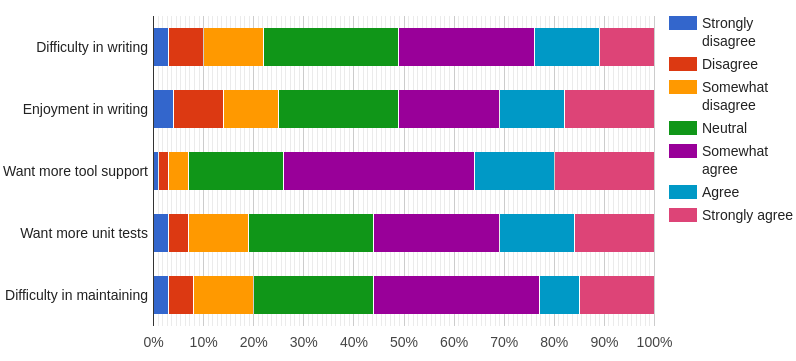
\includegraphics[width=14.7cm]{images/perception-org.png}
        \caption{Original study~\cite{daka2014survey} developer perception of unit testing}
        \label{fig:org-perception}
      \end{center}
    \end{figure}

Daka and Fraser~\cite{daka2014survey} have studied developer perception towards traditional unit testing. Interesting
points that are further studied for low-level testing in this study are shown in figure \ref{fig:org-perception}. Some
aspects to highlight are the facts that only about 50\% of survey responders \textit{enjoy writing} unit tests to some degree.
One of the hypothesis in this study was that implementation level BDD testing frameworks should increase low-level testing enjoyment.
Another interesting aspect is the \textit{difficulty in maintaining} unit tests, where around 55\% of study participants
feel maintaining at least somewhat difficult. One of the study hypothesis was that BDD testing frameworks should
make it less difficult to maintain code and especially the test code. Table \ref{tab:changes-pt11} displays the \textbf{Q14}, which studies
the developer perception towards low-level testing using Daka and Fraser's survey question as a base.

\textbf{Q15a} in table \ref{tab:changes-pt11} studies the developer perception aspect further. Its questions have originally
been used individually in two different studies~\cite{williams2009effectiveness}~\cite{li2016automatically}. The original
questions and their answers are displayed in figure \ref{fig:org-perception-two}. Interesting fact was that over 90\% of
original survey respondents feel that unit tests help in producing higher quality code than without them~\cite{williams2009effectiveness}.
Around same 90\% of different study participants feel that maintaining unit tests is important for system quality~\cite{li2016automatically}.

    \begin{figure}[ht]%
        \centering
        \subfloat[Unit tests help in producing higher quality code~\cite{williams2009effectiveness}]{{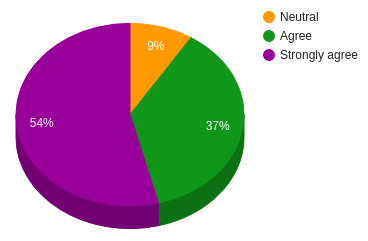
\includegraphics[width=6.75cm]{images/org-quality.png} }}%
        \qquad
        \subfloat[Maintaining unit tests is important for the quality of the system~\cite{li2016automatically}]{{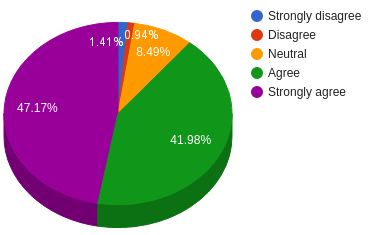
\includegraphics[width=6.75cm]{images/org-maintaining.png} }}%
        \caption{Developer perception of unit testing in original studies}%
        \label{fig:org-perception-two}%
    \end{figure}

Participants in this study based on their perception towards low-level automated testing with JUnit can be divided into
to category. Participants A and B are close to each other, they feel that
\textit{writing} low-level tests is somewhat difficult, \textit{enjoyment} in writing is neutral or negative and \textit{maintaining}
of low-level tests is seen at least somewhat difficult. They both still have trust that low-level testing is \textit{helpful in
finding defects}, but \textbf{don't} feel that JUnit \textit{promotes to write high quality test code}. Participants
A and B seem to fall into same category as majority of respondents in the original research.

Participant C could be categorized into a testing oriented developer when inspecting perception towards
low-level testing. He enjoys \textit{writing} low-level tests and doesn't find it that difficult. He also doesn't find
\textit{maintaining} low-level tests too difficult. He thinks that low-level tests that he has written with JUnit will \textit{help} others \textit{understanding}
the implemented production code. Like other participants, participant C also trusts that low-level
tests will \textit{help in finding defects}, but he \textbf{doesn't} feel that JUnit \textit{promotes him to write high quality} test code.

Although all study participants feel that JUnit doesn't promote in writing higher quality test code, all of them still
believe that low-level tests \textit{help in producing higher quality code}. They all feel that \textit{maintaining}
low-level tests and their documentation is important for the system quality. All of the participants seem to follow the
majority of developers in previous researches regarding test helping in quality and test maintaining importance.
Table \ref{tab:changes-pt11} displays the detailed answers of participants.

    \begin{table}[H]
        \resizebox{\textwidth}{!}{%
            \begin{tttabular}{p{8.0cm}*{7}{p{1.7cm}}}
            \topline
            \textbf{Question} & \textbf{Answer options} &  &  &  &   &  & \\ \hline

            \textbf{Q14: Please indicate your level of agreement with the following statements} & Strongly disagree & Disagree & Somewhat disagree & Neither agree nor disagree & Somewhat agree & Agree & Strongly agree \\
            & \\
            1. Writing low-level tests is difficult & & & {\colorbox{orange}C} & & {\colorbox{lightgray}A}{\colorbox{lime}B} & & \\
            2. I enjoy writing low-level tests & & {\colorbox{lime}B} & & {\colorbox{lightgray}A} & & {\colorbox{orange}C} & \\
            3. I would like to have more tool support when writing low-level tests & & & {\colorbox{lime}B} & {\colorbox{lightgray}A} & {\colorbox{orange}C} & & \\
            4. I would like to have more low-level tests & & & & {\colorbox{lightgray}A}{\colorbox{lime}B}{\colorbox{orange}C} & & & \\
            5. Maintaining low-level tests is difficult & & & {\colorbox{orange}C} & & {\colorbox{lime}B} & {\colorbox{lightgray}A} & \\
            6. I think my low-level tests will help other developers to understand the implemented unit/feature better & & & {\colorbox{lime}B} & & {\colorbox{lightgray}A} & {\colorbox{orange}C} & \\
            7. Low-level automated testing helps me find defects in the code before other quality assurance phases & & & & & {\colorbox{lime}B} & {\colorbox{orange}C} & {\colorbox{lightgray}A} \\
            8. JUnit promotes me to write high quality test code & & & {\colorbox{lightgray}A}{\colorbox{orange}C} & {\colorbox{lime}B} & & & \\
            & \\ \hline

            \textbf{Q15a: Please indicate your level of agreement with the following statements} & Strongly disagree & Disagree & Neutral & Agree & Strongly agree & \\
            & \\
            1. Overall, low-level tests help me produce higher quality code & & & & {\colorbox{lime}B} & {\colorbox{lightgray}A}{\colorbox{orange}C} \\
            2. Maintaining good low-level test cases and their documentations is important to the quality of a system & & & & {\colorbox{lightgray}A}{\colorbox{lime}B} & {\colorbox{orange}C} \\
            & \\ \topline

            \end{tttabular}}
            \caption {Developer perception of low-level testing with JUnit} \label{tab:changes-pt11}
    \end{table}

Table \ref{tab:changes-pt12} display questions \textbf{Q14'} and \textbf{Q15a'} together with their results. With \textbf{\textit{Spectrum}}
there exists some controversial and interesting results. Participant A somewhat agrees that \textit{writing}
and \textit{maintaining} of low-level tests with Spectrum is more difficult than with JUnit.
Writing difficulty was further analyzed in
the interview, where he states that the learning curve how to structure code example groups and code examples was still ongoing.
Also what to write in \textit{describe}-blocks was somewhat difficult. Slight increase in difficulty in maintaining low-level
tests with Spectrum comes from the use of example groups properly, as participant A feels that it
isn't always straightforward. In spite of slightly harder maintenance in total, he feels that it is easier to reduce repetition
with Spectrum's \textit{lifecycle hooks}.

Although writing and maintenance were found slightly harder, participant A somewhat agrees that he \textit{enjoys} writing low-level
tests with Spectrum more than with JUnit. He also thinks that Spectrum allows other developers to \textit{understand} the production
code better than earlier with JUnit. Participant A feels that Spectrum \textit{promotes him to write higher quality test code} than
JUnit. In addition, he felt that \textit{maintaining} of Spectrum tests was somewhat more important for system quality, but
didn't see Spectrum helping in producing hiqher quality production code.

    \begin{table}[H]
        \resizebox{\textwidth}{!}{%
            \begin{tttabular}{p{8.0cm}*{7}{p{1.7cm}}}
            \topline
            \textbf{Question} & \textbf{Answer options} &  &  &  &   &  & \\ \hline
            \textbf{Q14'\&Q15a': Please indicate your level of agreement with the following statements} & Strongly disagree & Disagree & Somewhat disagree & Neither agree nor disagree & Somewhat agree & Agree & Strongly agree \\
            & \\
            1. Writing low-level tests with \textit{Spectrum/Spock} is more difficult than with JUnit & & {\colorbox{orange}C} & & & {\colorbox{lightgray}A} & {\colorbox{lime}B} & \\
            2. I enjoy writing low-level tests with \textit{Spectrum/Spock} more than I do with JUnit & & & & {\colorbox{lime}B} & {\colorbox{lightgray}A} & {\colorbox{orange}C} & \\
            3. I would like to have more tool support for \textit{Spectrum/Spock} when writing low-level tests & & & & {\colorbox{orange}C} & & {\colorbox{lime}B} & {\colorbox{lightgray}A} \\
            4. I would like to have more low-level tests with \textit{Spectrum/Spock} & & & & {\colorbox{lime}B} & {\colorbox{lightgray}A}{\colorbox{orange}C} & & \\
            5. Maintaining low-level tests with \textit{Spectrum/Spock} is more difficult than with JUnit & & {\colorbox{orange}C} & & {\colorbox{lime}B} & {\colorbox{lightgray}A} & & \\
            6. I think my low-level tests with \textit{Spectrum/Spock} will help other developers to understand the implemented unit/feature better than earlier tests with JUnit & & & & {\colorbox{lime}B} & & {\colorbox{lightgray}A}{\colorbox{orange}C} & \\
            7. Low-level automated testing with \textit{Spectrum/Spock} helps me find defects in the code before other quality assurance phases better than earlier tests with JUnit & & &  {\colorbox{lightgray}A}{\colorbox{lime}B} & {\colorbox{orange}C} & & & \\
            8. \textit{Spectrum/Spock} promotes me to write higher quality test code than with JUnit & & {\colorbox{lime}B} & & & &  {\colorbox{lightgray}A}{\colorbox{orange}C} & \\ \hline
            & \\
            9. Overall, low-level tests with \textit{Spectrum/Spock} help me produce higher quality code than with JUnit & & {\colorbox{lime}B} &  {\colorbox{lightgray}A} & & {\colorbox{orange}C} & & \\
            10. Maintaining good low-level test cases and their documentation with \textit{Spectrum/Spock} is more important for system quality than maintaining JUnit test cases & & {\colorbox{lime}B} & & & {\colorbox{lightgray}A}{\colorbox{orange}C} & & \\
            & \\ \topline

            \end{tttabular}}
            \caption {Developer perception changes in low-level testing with \textit{Spectrum/Spock}} \label{tab:changes-pt12}
    \end{table}

Participant B finds \textit{writing} of low-level tests with Spectrum more difficult than with JUnit. This was further studied in the interview,
where he said that quite much of the trouble in writing came from Java features used to write Spectrum tests, but also one cause was the more difficult
structuring of tests. Both participants A
and B agree or strongly agree that they would like to have \textit{more tool support} for Spectrum. This was studied in following interviews,
where both would like to see more IDE support. For most of the statements, participant B neither agrees nor disagrees. He
disagrees with the statement that \textit{Spectrum promotes to write higher quality test code than JUnit}. This was further
discussed in the interview, where he says that he feels that the test case structure with Spectrum is more complex than
with JUnit. Participant B disagreed with statements that Spectrum \textit{helps producing higher quality production code} than JUnit
or that \textit{maintaining} Spectrum tests would be \textit{more important} for system quality.

Participant C disagreed that \textit{writing} and \textit{maintaining} of low-level tests with Spock is more difficult than with JUnit.
In the following interview, he stated that writing tests was quick to learn and they could be more easily divided
into logical parts with \textit{Given-When-Then} blocks. It is interesting to see that participant C initially already
\textit{enjoyed} writing low-level tests with Junit and agreed to \textit{enjoy} even more low-level testing with Spock.
With Spock, he also feels that other developers will \textit{understand} the implemented unit or feature better than with JUnit.
Participant C agrees that all in all Spock \textit{promotes} him to write higher quality test code}. In total, participant C
seemed to perceive Spock well, as he also somewhat agrees that Spock \textit{helps to produce overall higher quality code} and that
\textit{maintaining} of Spock tests is more important for system quality.

Table \ref{tab:changes-pt13} displays question \textbf{Q15b} and its answers. Q15b holds two sub-question statements that the participant can answer
if they feel the same way or not. Sub-question 1 relates directly to hypothesis 2 and sub-question 2 to
hypothesis 3. Participant A and C feel that they write both more \textit{understandable} and more \textit{maintainable} low-level
tests with Spectrum and Spock than with JUnit. Participant B on the other hand feels neither sub-question statements
to be true. In the feedback interview, these questions were further studied. Participant B feels that Spectrum has just a
different way of doing things than JUnit and both have their areas where they perform better than the other.

    \begin{table}[H]
        \resizebox{\textwidth}{!}{%
            \begin{tttabular}{p{15.0cm}*{3}{p{2.0cm}}}
            \topline
            \textbf{Question} & \textbf{Answer options} &  &  \\ \hline

            \textbf{Q15b: I would say that I write more} & Yes & Uncertain & No \\
            & \\
            1. Understandable low-level tests with \textit{Spectrum/Spock} than with JUnit? & {\colorbox{lightgray}A}{\colorbox{orange}C} & & {\colorbox{lime}B} \\
            2. Maintainable low-level tests with \textit{Spectrum/Spock} than with JUnit? & {\colorbox{lightgray}A}{\colorbox{orange}C} & & {\colorbox{lime}B} \\
            & \\ \topline

            \end{tttabular}}
            \caption {Developer perception towards \textit{Spectrum/Spock}} \label{tab:changes-pt13}

    \end{table}

Many of the made hypotheses get support from these results.
\textbf{H2:} \textit{"Developers will find it easier to understand test cases"} seems to have more evidence as two out of
three participants find test cases more understandable. \textbf{H3:} \textit{"Developers will find it easier to maintain code"}
has some results supporting it. Only Spock tests were perceived as easier to maintain than JUnit ones, but both Spectrum
and Spock had developers that felt new tests with BDD testing frameworks would act as easier to understand documentation for the
production code. This living documentation is one the claims of BDD literature~\cite{smart2014bdd} and it seems to have
merit. In total, H3 seems to hold true to an extent.
\textbf{H4:} \textit{"Developers will perceive working with low-level automated testing more enjoyable"} has two out
of three developers agreeing with the statement. This could be interesting to study in a larger scale, as low enjoyment~\cite{daka2014survey}
and motivation~\cite{runeson2006survey} in unit testing was found problematic in earlier researches. With the results from
this study, it can't be said with certainty that BDD testing frameworks are the answer for enjoyment problem. Although
there is more evidence to support H4 than not.


Summing up, participants A and C could be grouped closer together regarding developer perception changes with BDD testing
frameworks. This is somewhat interesting, as they use different frameworks. In total, the changes in their perception could be categorized
to be on the positive side. Participant B could be categorized to perceive the change as indifferent or negative. Its interesting
to see that participants A and B have same kind of experience as developers and they perceive low-level testing with JUnit the same,
but the difference in perceiving the Spectrum changes is quite different.


\subsubsection{Developer loyalty towards low-level testing}
Developer loyalty towards low-level testing is measured with \textbf{NPS} survey questions. As the participant count is so low, it is not
sensible to calculate the NPS directly. The information what can be used, is that for every sub-question in questions
\textbf{Q16} and \textbf{Q16'} values from zero to six are called \textit{detractors}, seven to eight \textit{passives} and
nine to ten \textit{promoters}~\cite{reichheld2003one}. The interesting part here is to see, whether the participant has gained loyalty enough
towards testing framework to be called a promoter.

    \begin{table}[H]
        \resizebox{\textwidth}{!}{%
            \begin{tttabular}{p{10.0cm}*{11}{p{0.75cm}}}
            \topline
            \textbf{Question} & \multicolumn{3}{l}{\textbf{Answer options}} & \\
            & \\ \hline
            & \multicolumn{4}{l}{\textit{Not at all likely}} & & & & \multicolumn{4}{r}{\textit{Extremely likely}} \\
            \textbf{Q16: How likely are you to} & 0 & 1 & 2 & 3 & 4 & 5 & 6 & 7 & 8 & 9 & 10 \\
            & \\
            1. Recommend low-level automated testing for colleague as a software development practice? & & & & & & & & & {\colorbox{lime}B} & & {\colorbox{lightgray}A}{\colorbox{orange}C} \\
            2. Recommend testing framework JUnit for future Spring projects where you take part in existing project? & & & & & & & & {\colorbox{orange}C} & & {\colorbox{lime}B} & {\colorbox{lightgray}A} \\
            3. Take testing framework JUnit in use for future Spring projects where you have technical lead role in a new starting project? & & & & & & & & & {\colorbox{orange}C} & {\colorbox{lime}B} & {\colorbox{lightgray}A} \\
            & \\ \hline
            & \multicolumn{4}{l}{\textit{Not at all likely}} & & & & \multicolumn{4}{r}{\textit{Extremely likely}} \\
            \textbf{Q16': How likely are you to} & 0 & 1 & 2 & 3 & 4 & 5 & 6 & 7 & 8 & 9 & 10 \\
            & \\
            1. Recommend low-level automated testing for colleague as a software development practice? & & & & & & & & & {\colorbox{lime}B} & & {\colorbox{lightgray}A}{\colorbox{orange}C} \\
            2. Recommend testing framework \textit{Spectrum/Spock} for future Spring projects where you take part in existing project? & & & & {\colorbox{lime}B} & & & {\colorbox{lightgray}A} & & {\colorbox{orange}C} & & \\
            3. Take testing framework \textit{Spectrum/Spock} in use for future Spring projects where you have technical lead role in a new starting project? & & & & {\colorbox{lime}B} & & & {\colorbox{lightgray}A} & & {\colorbox{orange}C} & & \\
            & \\ \topline

            \end{tttabular}}
            \caption {NPS questions related to JUnit and \textit{Spectrum/Spock}} \label{tab:changes-pt14}

    \end{table}

Table \ref{tab:changes-pt14} displays all the NPS survey questions with answers.
Participants A and C can be categorized as promoters of low-level testing
in general before and after the introduction of new BDD testing framework. Participant B remains as a
passive before and after the change.

Before the introduction of \textbf{\textit{Spectrum}}, participant A
is also a steady promoter of JUnit both as a technical lead in new project or taking part in existing project. After
using Spectrum for two months, participant can be categorized as a detractor in loyalty towards Spectrum in \textit{Spring Framework} context.
This was further
analyzed in interview where participant states that the found bugs in 1.1.0 version of Spectrum in IDE test output and build test output
lower the score. He also states that \textit{Spring Framework} support is not optimal yet and for these reasons he hesitates
to fully get on board with Spectrum.
The same effect is visible with participant B, as he was first a promoter of JUnit, but can later be categorized as a detractor for Spectrum NPS.
In the interview he says that the lacking \textit{Spring Framework} support is the main reason for not recommending Spectrum.
Participant C remains as a passive both with JUnit and Spock, although he states in following interview that he would more
probably use Spock in a new \textit{Spring Framework} project than JUnit.

\subsubsection{Change summary}

{\renewcommand{\arraystretch}{1.3}
\begin{table}[H]
    \resizebox{\textwidth}{!}{%
        \begin{tabular}{p{10.0cm}p{5cm}}

        \headcol \textbf{Benefit} & \textbf{Participants agreeing} \\ \hline

        \rowcol Easier to write tests & C \\
        Enjoy writing tests & A, C \\
        \rowcol Maintaining is easier & C \\
        Tests help to understand production code better & A, C \\
        \rowcol Promotes to write higher quality test code & A, C \\
        More understandable tests & A, C \\
        \rowcol More maintainable tests & A, C \\
        & \\
        \headcol \textbf{Drawback} & \\ \hline
        \rowcol More difficult to write tests  & A, B \\
        Slightly more diffucult to maintain tests & A \\
        \rowcol Would like to have more tool support & A, B \\
        Early version & A, B \\
        \end{tabular}}
        \caption {Developer perception changes of low-level testing} \label{tab:practice-change}
\end{table}
}

\clearpage

\section{Test code analysis}
Test code analysis was done to answer \textbf{RQ3} with metrics defined in chapter \ref{chapter:methods} section \ref{subsub:test}.
Test code analysis was done with master branches of projects A and B, \textbf{before} and \textbf{after} the introduction of new BDD testing framework, to related
low-level tests and their affected components. First the unit testing level changes are inspected with projects A and B.
After this, the low-level testing metrics and changes in them are demonstrated with both projects. Finally, the findings are summarized.

\subsection{Automated unit testing level}
\label{subsub:unit-level-metrics}
At automated unit testing level, two metrics were used to study the changes in unit testing: average \textbf{count of test methods}
per tested class methods and \textbf{code coverage}. Table \ref{tab:unit-metrics} displays these values before the introduction
of new BDD testing framework and after. In \textbf{COTM} before values were calculated for JUnit unit tests only and after
values only for new unit tests done with the selected BDD testing framework. In \textbf{CC}, before values are for the
whole project at unit level with JUnit. After values are unit testing coverage for JUnit and new BDD testing framework
combined.

{\renewcommand{\arraystretch}{1.3}
\begin{table}[H]
    \resizebox{\textwidth}{!}{%
        \begin{tabular}{p{6.0cm}*{4}{p{3cm}}}

        \headcol \textbf{Metric} & \textbf{Project A} \newline JUnit & \textbf{Project A} \newline Spectrum & \textbf{Project B} \newline JUnit & \textbf{Project B} \newline Spock  \\ \hline

        \rowcol \textit{\textbf{COTM}} & \textbf{1.44} & \textbf{5.63} & \textbf{3.49} & \textbf{25.5}  \\
        \rowcol \textit{Sum of tested class methods} & 61 & 8 & 93 & 4 \\
        \rowcol \textit{Sum of unit test methods} & 88 & 45 & 325 (294)* & 102 (7)* \\ \hline

        \textit{\textbf{Instruction CC}} & \textbf{25\%} & \textbf{24\%} & \textbf{20\%} & \textbf{19\%} \\
        \textit{Total number of instructions} & 31,425 & 44,427 & 49,895 &  53,211 \\
        \textit{\textbf{Branch CC}} & \textbf{24\%} & \textbf{26\%} & \textbf{20\%} & \textbf{21\%} \\
        \textit{Total number of branches} & 724 & 1,107 & 2,195 & 2,316 \\ \bottomlinec
        \end{tabular}}
        \caption {Unit level testing metrics in projects and their change} \label{tab:unit-metrics}
        \caption*{* = Value in parenthesis is without calculating data-driven tests sum}
\end{table}
}

\begin{figure}[ht]
  \begin{center}
    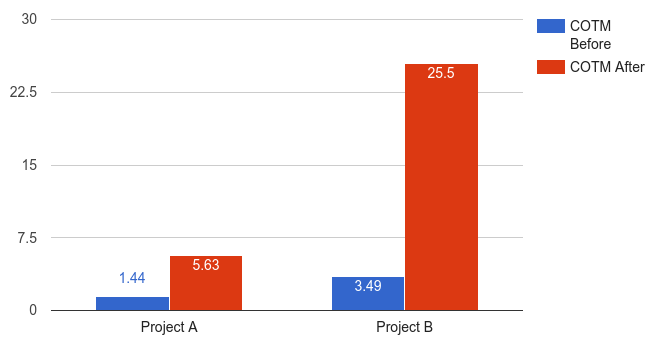
\includegraphics[width=12.7cm]{images/COTM.png}
    \caption{Average count of unit test methods per tested class method in projects}
    \label{fig:cotm}
  \end{center}
\end{figure}

\textbf{RQ3: }\textit{How does behavior-driven testing frameworks change written low-level test cases and test code coverage compared to JUnit framework?}
is first studied with data from unit testing metrics displayed in table \ref{tab:unit-metrics}. Figure \ref{fig:cotm} visualizes
the change in \textbf{COTM}. Both projects display a \textbf{drastic change} in number of unit test methods per tested class method. With JUnit, project A
had around one to two unit test methods per class method, but with Spectrum the average is from 5 to 6 test methods per class method. The
change is around 4 times more granular use of test methods than before. The change in COTM in project A seems to correlate well with the original
claims of Astels~\cite{astels2006new}: \textit{xSpec family} testing helps in producing more granular tests without the tight one-to-one mapping of test methods
to class methods.

At the starting point with JUnit, project B had first a fair amount of around 3 to 4
test methods per tested class method. With Spock, the average count of unit test methods per tested
class method is at staggering 25 to 26 methods. In total there were 7 unit level feature methods with Spock, but all of them were
data-driven tests. This resulted in 102 automatically generated separate test runs. As the number of study participants with Spock is low, this COTM-value might
be an anomaly. Still, together with the later studied \textit{DDTM}-metric, the analysis displays
a significant growth in use DDT. The advertisement of Spock's easy automatic test generation with DSL for data-driven testing~\cite{kapelonis2016java}
seems to have merit.

Both of studied BDD testing frameworks showed an increase in test case granularity with test code analysis and participant practice
survey. With the given study sample, \textbf{H1:} \textit{"Developers will write more granular test cases"} holds true.
This results in separately passing or failing test runs. In the original situation, less granular test cases could hold potentially multiple
assertion errors at single test method run, but the first one halts the run of that test method. More granular test cases including more separate
test methods with behavior describing naming should help in finding the erroneous situation faster.

\textbf{Code coverage} didn't show almost any changes at unit level in either project. As participants earlier answered in the survey, none
of them had code coverage as an optimizing target for low-level tests. This could explain the low coverage percentage seen in
table \ref{tab:unit-metrics}. Although the test case granularity has risen a lot in both projects, it doesn't
show up in test coverage one way or another. As such, it seems that CC is a poor metric to analyze changes in actual test
code. This is further confirmed in next section with low-level test coverage examination.

\subsection{Automated unit \& integration testing levels}
\label{subsub:low-level-metrics}
At automated low-level testing level there were 5 inspected metrics: \textbf{code coverage}, average \textbf{count of assertions} per test method,
average \textbf{count of comments} per test method, average \textbf{test method name word count} and ratio of \textbf{data driven test methods} to
all low-level test methods. \textbf{CC} was measured as combined JUnit and new BDD framework coverage. All other metrics
were measured first from existing low-level JUnit tests and after from new BDD testing framework specifications.
Table \ref{tab:low-metrics} dislays the values of these metrics in projects A and B before and after introduction of BDD testing framework.


{\renewcommand{\arraystretch}{1.3}
\begin{table}[H]
    \resizebox{\textwidth}{!} & \textbf{58\%} & \textbf{47\%} & \textbf{46\%} \\
        \rowcol \textit{Total number of instructions} & 31,425 & 44,427 & 49,895 & 53,211 \\
        \rowcol \textit{\textbf{Branch CC}} & \textbf{54\%} & \textbf{54\%} & \textbf{39\%} & \textbf{40\%} \\
        \rowcol \textit{Total number of branches} & 724 & 1,107 & 2,195 & 2,316 \\ \hline

        \textit{\textbf{COA}} & \textbf{2.64} & \textbf{2.07} & \textbf{2.82} & \textbf{2.46} \\
        \textit{Sum of assertions} & 493 & 174 & 1,311 & 32 \\
        \textit{Sum of test methods} & 187 & 84 & 465 & 13 \\ \hline

        \rowcol \textit{\textbf{COC}} & \textbf{1.17} & \textbf{0.08} & \textbf{0.04} & \textbf{0.07} \\
        \rowcol \textit{Sum of comments} & 218 & 7 & 20 & 1 \\
        \rowcol \textit{Sum of test methods} & 187 & 84 & 465 & 13 \\ \hline

        \textit{\textbf{TMNWC}} & \textbf{4.66} & \textbf{11.29} & \textbf{5.61} & \textbf{8.08} \\
        \textit{Total words in test method names} & 872 & 948 & 2,607 & 105 \\
        \textit{Sum of test methods} & 187 & 84 & 465 & 13 \\ \hline

        \rowcol \textit{\textbf{DDTM}} & \textbf{0} & \textbf{0}  & \textbf{0.02} & \textbf{0.54} \\
        \rowcol \textit{Sum of data driven test methods} & 0 & 0 & 8 & 7 \\
        \rowcol \textit{Sum of test methods} & 187 & 84 & 465 & 13  \\ \bottomlinec

        \end{tabular}}
        \caption {Low-level testing metrics in projects and their change} \label{tab:low-metrics}

\end{table}
}

\textbf{RQ3} can be further analyzed for low-level testing with metrics displayed in table \ref{tab:low-metrics}.
First studied metric is \textbf{CC}. With combined JUnit unit and integration tests, the instruction and branch coverage rises in both projects
to around 50\%. After the introduction of BDD testing frameworks in projects, the combined CC  \newgeometry{left=2.9cm, right=2.9cm} \noindent for JUnit and new BDD tests remain
virtually identical. It can be concluded, that although other studied metrics show quite significant changes, CC remains
unchanged.

Figure \ref{fig:coa-coc} part a. displays the change in \textbf{COA} after the introduction of BDD testing frameworks. Both of projects had closer to three
than two assertions per test method with JUnit. With Spectrum, project A displayed a drop to approximately
two assertions
per test method. This is natural reaction to the more granular test cases - now there are more test methods that contain
less assertions per method than before. The total count of assertions show an upward trend to earlier, as the total of 84 low-level
test methods are a sum from far less test files (14 pcs.) than before (53 pcs. with JUnit).

Project B displayed smaller change in COA after the introduction of Spock. It is hard to say whether there would be a significant
change in this with larger sample of test files to analyze. The structure of Spock, having assertions in \textit{Then}-blocks,
do not separate assertions to individual feature methods, instead one method can hold multiple blocks~\cite{spock}. How
this would affect COA in the long run, remains uncertain from these results.

    \begin{figure}[H]%
        \centering
        \subfloat[Average count of assertions per test method]{{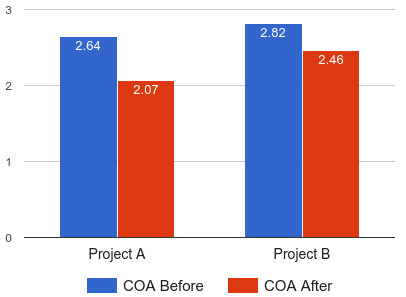
\includegraphics[width=7cm]{images/COA.png} }}%
        \qquad
        \subfloat[Average count of comments per test method]{{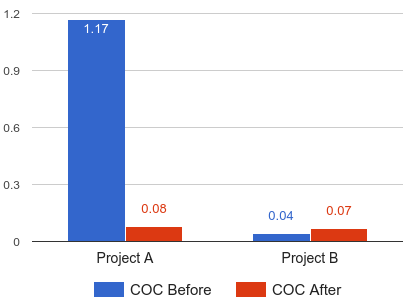
\includegraphics[width=7cm]{images/COC.png} }}%
        \caption{Test assertions and comments in projects}%
        \label{fig:coa-coc}%
    \end{figure}

Figure \ref{fig:coa-coc} part b. shows the change in \textbf{COC} in projects. Commenting test cases and updating those
comments was a practice that was found rarely done in earlier research~\cite{li2016automatically}. Compared to this,
project A showed to be an exception earlier with JUnit, as there was approximately atleast one comment per test method.
After the introduction of Spectrum, there was interesting change in test method commenting. The count of actual comments
in tests dropped drastically to almost average zero comments per test method. When inspecting the change in \textbf{TMNWC}
displayed in figure \ref{fig:tmnwc-ddtm} part a, there seems to be a correlation with the drastic change in test commenting
practices and the test naming practices. Info that was earlier inserted as pure comments, seem to be now a part of test
naming with \textit{describe} and \textit{it} blocks. This also allows that info to be a part of test output, so for instance
the failing test output could help the developer to grasp the test situation faster.

Project B with Spock showed virtually no change in commenting practices. There wasn't lot of commenting before and there still isn't
commenting in place in tests with Spock. Interesting to see, is that also the possible textual descriptions of \textit{Given-When-Then} blocks
were missing. The change in TMNWC in project B was about 50\% increase in test method name words, but as the block descriptions
are optional, it is interesting to ponder how much more Spock actually promotes to write textual info into tests than
JUnit. Unfortunately now, only one participant Spock testing habbits were studied.

Earlier study~\cite{li2016automatically} had identified developers preferring the tests to be self-document- ing without commenting.
Together with COC and TMNWC from both projects, there seems to be evidence to say that both BDD testing frameworks
promote this aspect better than JUnit. The text descriptions as part of test method naming seems to promote this self-documenting
aspect of low-level tests. This is potentially more evidence for \textbf{H2:} \textit{"Developers will find it easier to understand test cases"}, at least
there exists less need for commenting of test methods and the test names hold more information through more words in them.
Together with earlier survey and interview results, it can be concluded that H2 seems to hold true to an extent.

    \begin{figure}[H]%
        \centering
        \subfloat[Average test method name word count]{{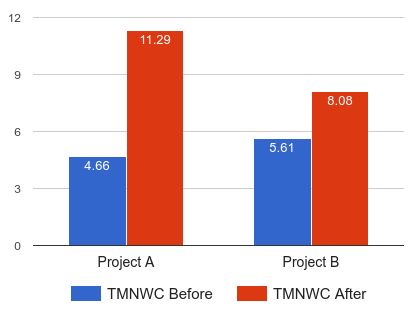
\includegraphics[width=7cm]{images/TMNWC.png} }}%
        \qquad
        \subfloat[Ratio of data-driven tests to standard low-level test methods]{{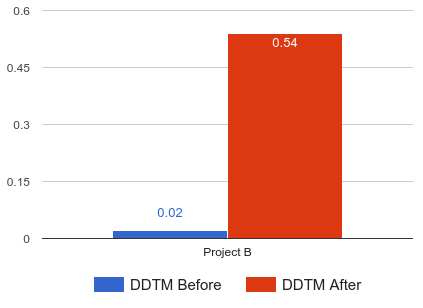
\includegraphics[width=7cm]{images/DDTM.png} }}%
        \caption{Test method naming and DDT in projects}%
        \label{fig:tmnwc-ddtm}%
    \end{figure}

\textbf{TMNWC} changes are displayed in figure \ref{fig:tmnwc-ddtm} part a. The relation between commenting practices
and TMNWC was already discussed, but it's still good to highlight that in project A with Spectrum, there is on average
almost 2.5 times words in test method names. The nested example groups and their code examples features in \textit{xSpec family} testing
seem to promote much better information on test method names than\restoregeometry \noindent  JUnit. In project B, Spock displayed only 50\% increase in TMNWC.
Tester habbits might be one of the reasons, but also the single line text description for test method naming could be a
reason for this more mild increase.

\textbf{DDTM} metrics can be seen in figure \ref{fig:tmnwc-ddtm} part b. Project A didn't have any DDT with JUnit at the start,
nor did it have after the introduction of Spectrum. Spectrum and Java 8-lambdas allow automatic test method generation with
usage through the language features, but the framework doesn't support this with DSL. Earlier with JUnit, Project B had about 2\% of
all low-level test methods as data-driven. After the introduction of Spock, there were a drastic change:
 54\% of all
feature methods were data-driven.
Spock seems to promote DDT really well with it's DSL and thus, at least maintaining of low-level tests with different
test conditions should be easier.

\subsection{Change summary}

{\renewcommand{\arraystretch}{1.3}
\begin{table}[H]
    \resizebox{\textwidth}{!}{%
        \begin{tabular}{p{6.0cm}*{2}{p{4cm}}}

        \headcol \textbf{Metric} & \textbf{Project A} & \textbf{Project B} \\ \hline

        \rowcol \textit{\textbf{COTM}} & ++ & +++ \\
        \textit{\textbf{CC}} & stagnant & stagnant \\
        \rowcol \textit{\textbf{COA}} & - & - \\
        \textit{\textbf{COC}} & - - - & stagnant \\
        \rowcol\textit{\textbf{TMNWC}} & +++ & + \\
        \textit{\textbf{DDTM}} & stagnant & +++ \\ \hline

        \end{tabular}}
        \caption {Test code analysis metrics change in projects} \label{tab:test-change}
        \caption*{+ = Increase amount, - = Decrease amount}
\end{table}
}

BDD testing frameworks introduced changes to almost all of the studied testing metrics. \textit{COTM} displayed a drastic change
in both projects and especially with Spock and its data-driven testing. Both frameworks promote a lot more granular
test cases than JUnit.

\textit{Code coverage} remained virtually unchanged after the introduction of BDD testing frameworks. In
hindsight, it was fairly uninteresting metric to study this kind of testing transformation. It might have had different
kind of results if actual BDD was practiced during the study.

\textit{COA} had decrease in both projects. With project B, the amount of test files to study was fairly low and thus it is
hard to draw real conclucions. Project A on the other hand displayed slightly more decrease in \textit{COA}. This seems natural
to the more granular use of test methods.

\textit{COC} showed a significant change in project A test commenting practices. Earlier with JUnit, test commenting was an often
used practice. After the introduction of Spectrum, this practice appeared to be substantially less used. Project B didn't
have regular test commenting practices with JUnit. Spock didn't change the fact and test commenting remained a practice
that was seldom used.

\textit{TMNWC} changed in both projects. Project A had almost 2.5 times increase test method name word count with Spectrum. In
project B, there was around 50\% increase in \textit{TMNWC}. Both BDD testing families seem to promote more information on test
names than JUnit. Spectrum and its internal structure seems to promote this even more than Spock. Together with the changes
in test method naming and commenting, compared to JUnit, BDD testing frameworks should produce more self-documenting test cases.

Data-driven testing was only in place in project B. Before with JUnit, DDT was used only a few times in total
of low-level testing. With Spock, \textit{DDTM}-metric increased tenfolds. Around half of the new tests with Spock were data-driven.
It can be concluded that Spock promotes the use of data-driven testing much more than JUnit.

Table \ref{tab:test-change} summarises the results for \textbf{RQ3} - the changes in written low-level test and code coverage.
The main findings are:

\begin{center}
\begin{topbot}
\textit{In low-level testing, BDD testing frameworks produce more granular and self-documenting test cases than JUnit.
Spock promotes the use of DDT more than JUnit.}
\end{topbot}
\end{center}

\section{Comparison summary of BDD testing frameworks}

